\chapter{Terminologies}

\begin{itemize}
	\item Le client est le commanditaire du projet.
	\item Un utilisateur est une personne souhaitant utiliser un logiciel du client. 
	\item Une licence est un droit accordé pour une machine et un utilisateur d'utiliser un logiciel donné.
	\item Craquer un logiciel est le fait de pouvoir l'utiliser sans avoir payé pour son utilisation. 
	Soit en modifiant le code compilé, soit en utilisant une autre méthode. 
\end{itemize}

\chapter{Présentation}

Le but de ce projet est de fournir une solution permettant de protéger les applications
du client sur Windows en évitant leur copie ou leur utilisation illégale. 
Il devra également permettre au client de générer et gérer des licences d'utilisations 
via une interface graphique. Il pourra ainsi définir des contraintes sur les licences 
comme par exemple leur durée de validité.\\
\begin{figure}[!h]
    \centering
    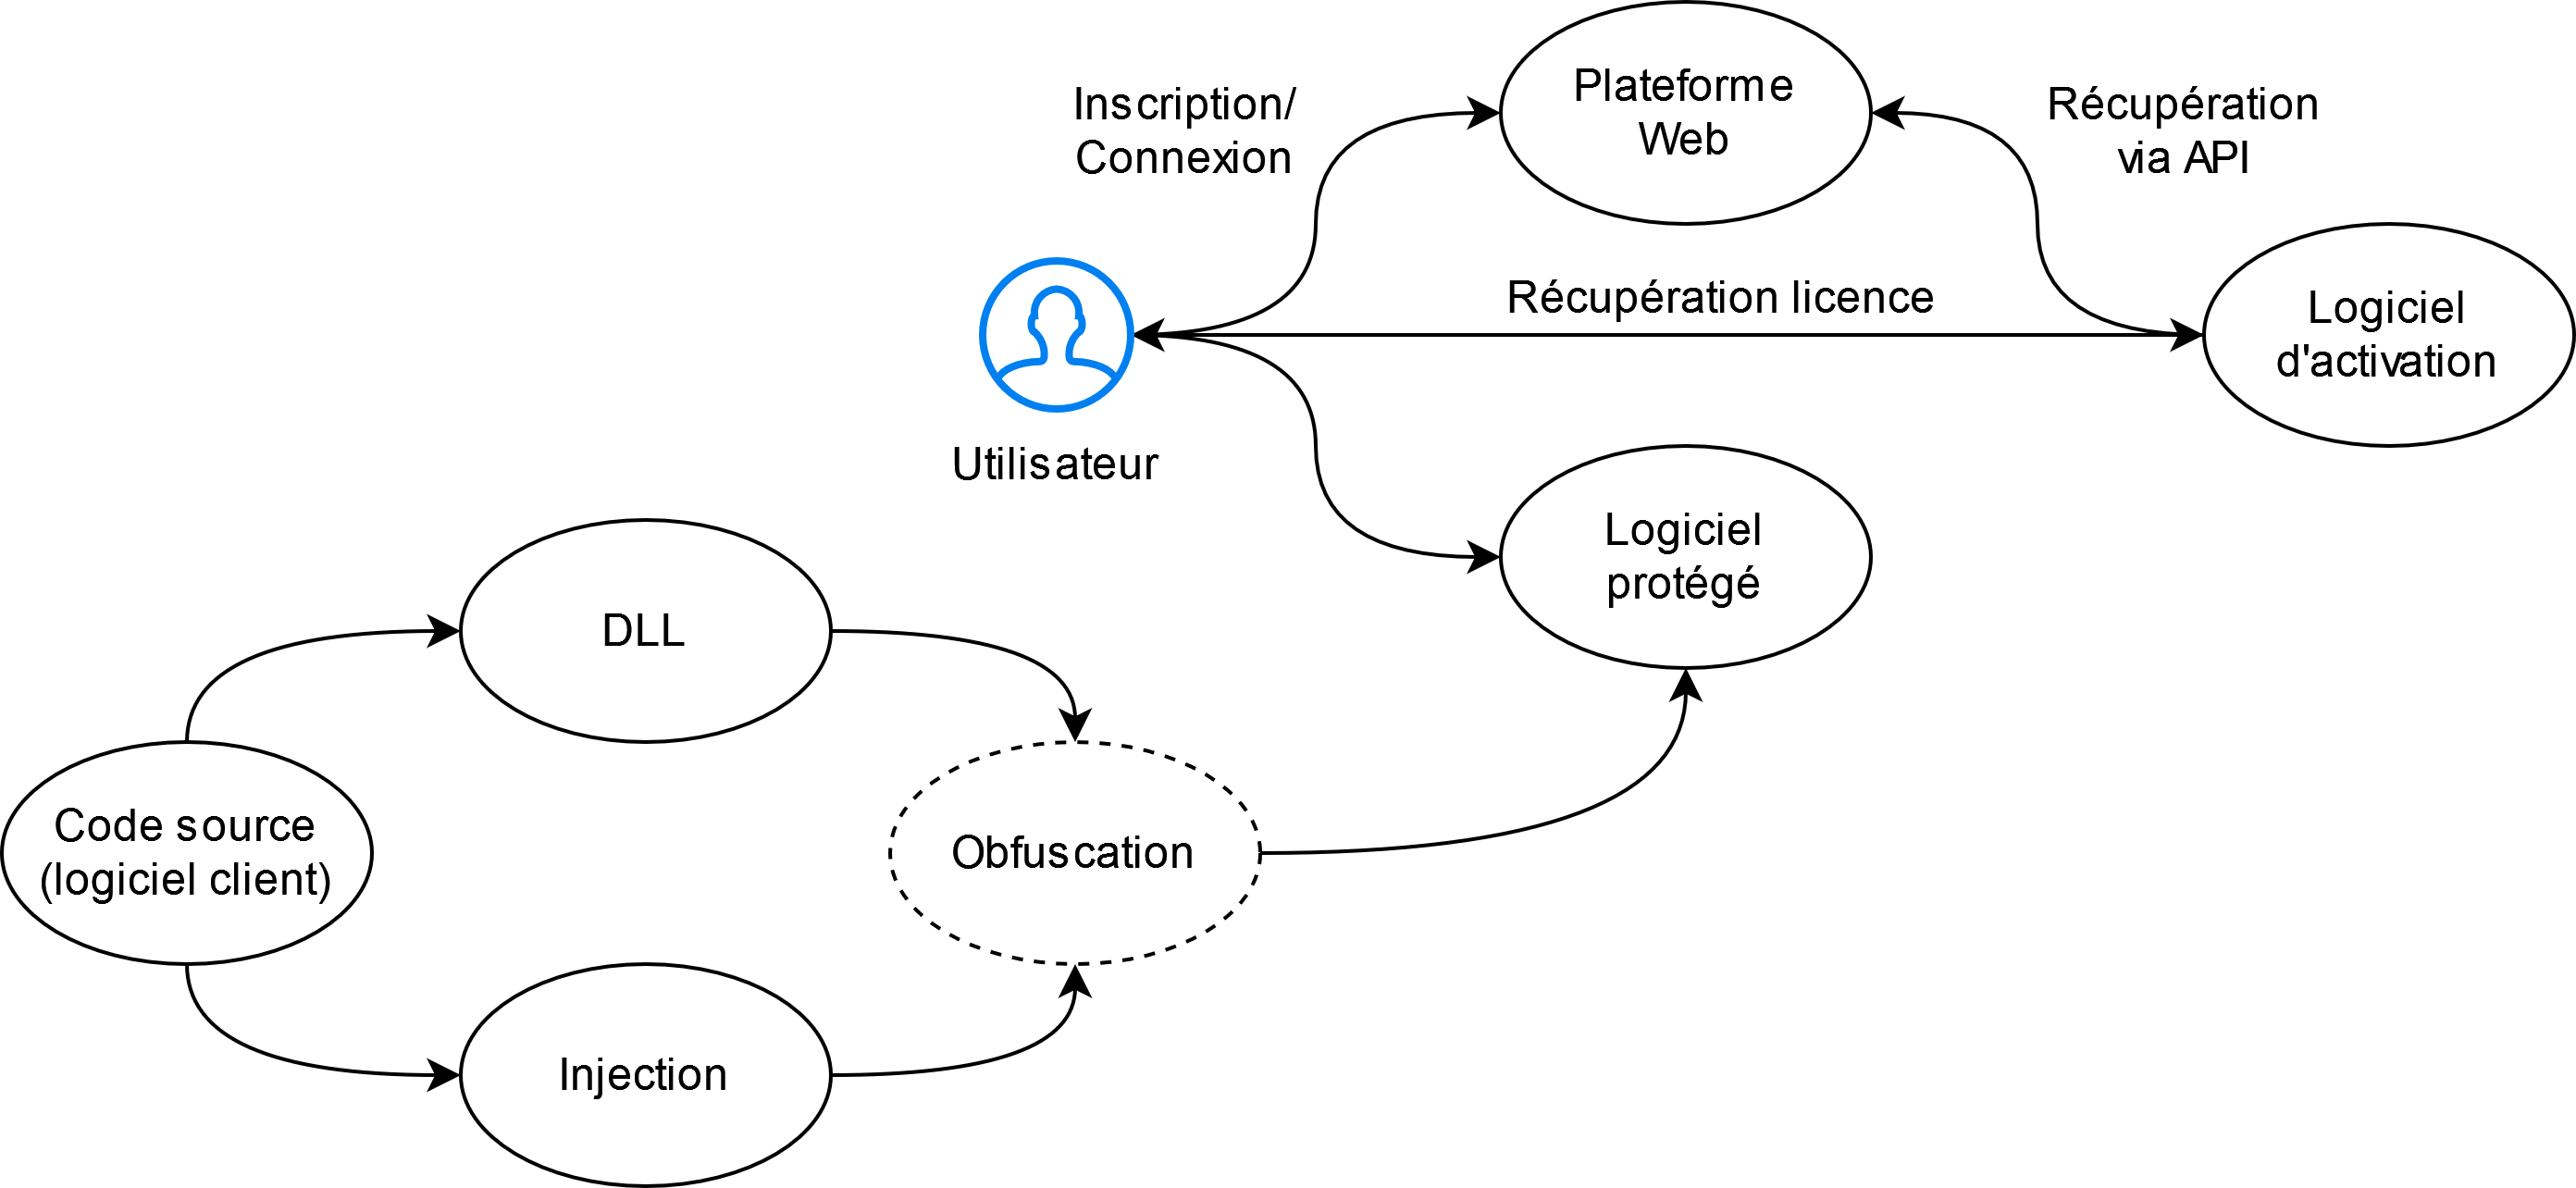
\includegraphics[width=12cm, scale=0.7]{general.png}
    {\small{\emph{\caption{fonctionnement général du projet}}}}
\end{figure}
Lors de ce projet nous avons mis en place un système de vérification de 
licence comprenant:
\begin{description}
    \item[\verb:DLL:] 
        Cette bibliothèque de fonctions permet de générer les informations
        lié au matériel d'un utilisateur, de l'envoyer au serveur puis de 
        vérifier un système de licence.
    \item[\verb:Plateforme web:] 
        Ce site permet aux clients de se créer un compte, 
        d'acheter des licences pour des logiciels et permet également à 
        l'administrateur de lister les demandes, de les accepter ou de 
        les refuser.
    \item[\verb:Logiciel d'activation:] 
        Ce logiciel permet de récuperer depuis la machine
        d'un client une licence pour un logiciel donné.
    \item[\verb:Algorithme de Détection de fraude:]
        Cette algorithme vérifie qu'un utilisateur nécessaie pas de modifier 
        le fichier de licence afin de s'accorder une plus grande durée d'utilisation. 
    \item[\verb:Documentation:]
        Nous avons également fournis une documentation complète de tous le code
        afin que celui-ci puisse être eventuellement repris dans les années à venir.
\end{description}

\chapter{Gestion de projet}

\section{Organisation}

Depuis le début du projet nous travaillons selon un fonctionnement agile, avec des
réunions et des livrables réguliers, avec le client qui se sont intensifiés au cours du semestre 2. Ce fonctionnement a permis de produire des livrables et de
la valeur rapidement.\newline

L'organisation de ce projet nous a permis de travailler efficacement, nous avions affecté un rôle à
chacun. Néanmoins, tous les acteurs de ce projet ont eu les rôles de développeur plus ou moins prononcé ainsi qu'un role de
rédacteur. Je me permet de vous renvoyer vers l'organigramme présenté dans le plan de développement en post production.\newline

Au cours de ce développement deux audits ont eu lieu. Cela nous a permis de comprendre les points forts mais surtout les points faibles de notre
organisation c'est pourquoi certain points ont été ajoutés/améliorés à celle-ci. \newline

Nous avons divisé la charge et la répartition par phase en méthode agile. La première phase était intitulée
«Préparation». Cette première phase a permis de donner un temps approximatif de structuration du
projet, de vérification des répartitions des tâches et des phases de tests ce qui a donné des
évaluations de temps de développement plus précises tel que les tests de greffe de code infructueux ou ceux
d'obfuscation. Cette phase a été suivis d'une phase de structure de projet avec le client qui a attester de la bonne évaluation de temps
et des ressources nécessaires. Après ca est venu la phase de développement. Nous avons donc suivis une méthode agile avec une période de sprint de 2 semaines, mais
celle-ci sera abordée plus en profondeur dans la prochaine section "Déroulement".\newline

\newpage

\section{Déroulement}

Le projet s'étant déroulé au cours de l'année scolaire l'organisation à du s'adapter aux
contrainte de temps de travail demandé par les autres matières ainsi qu'aux modifications d'emploie
du temps de chacun. Ce qui a donné ce diagramme de Gantt lors du second audit courant Avril.

\begin{figure}[!h]
	\centering
	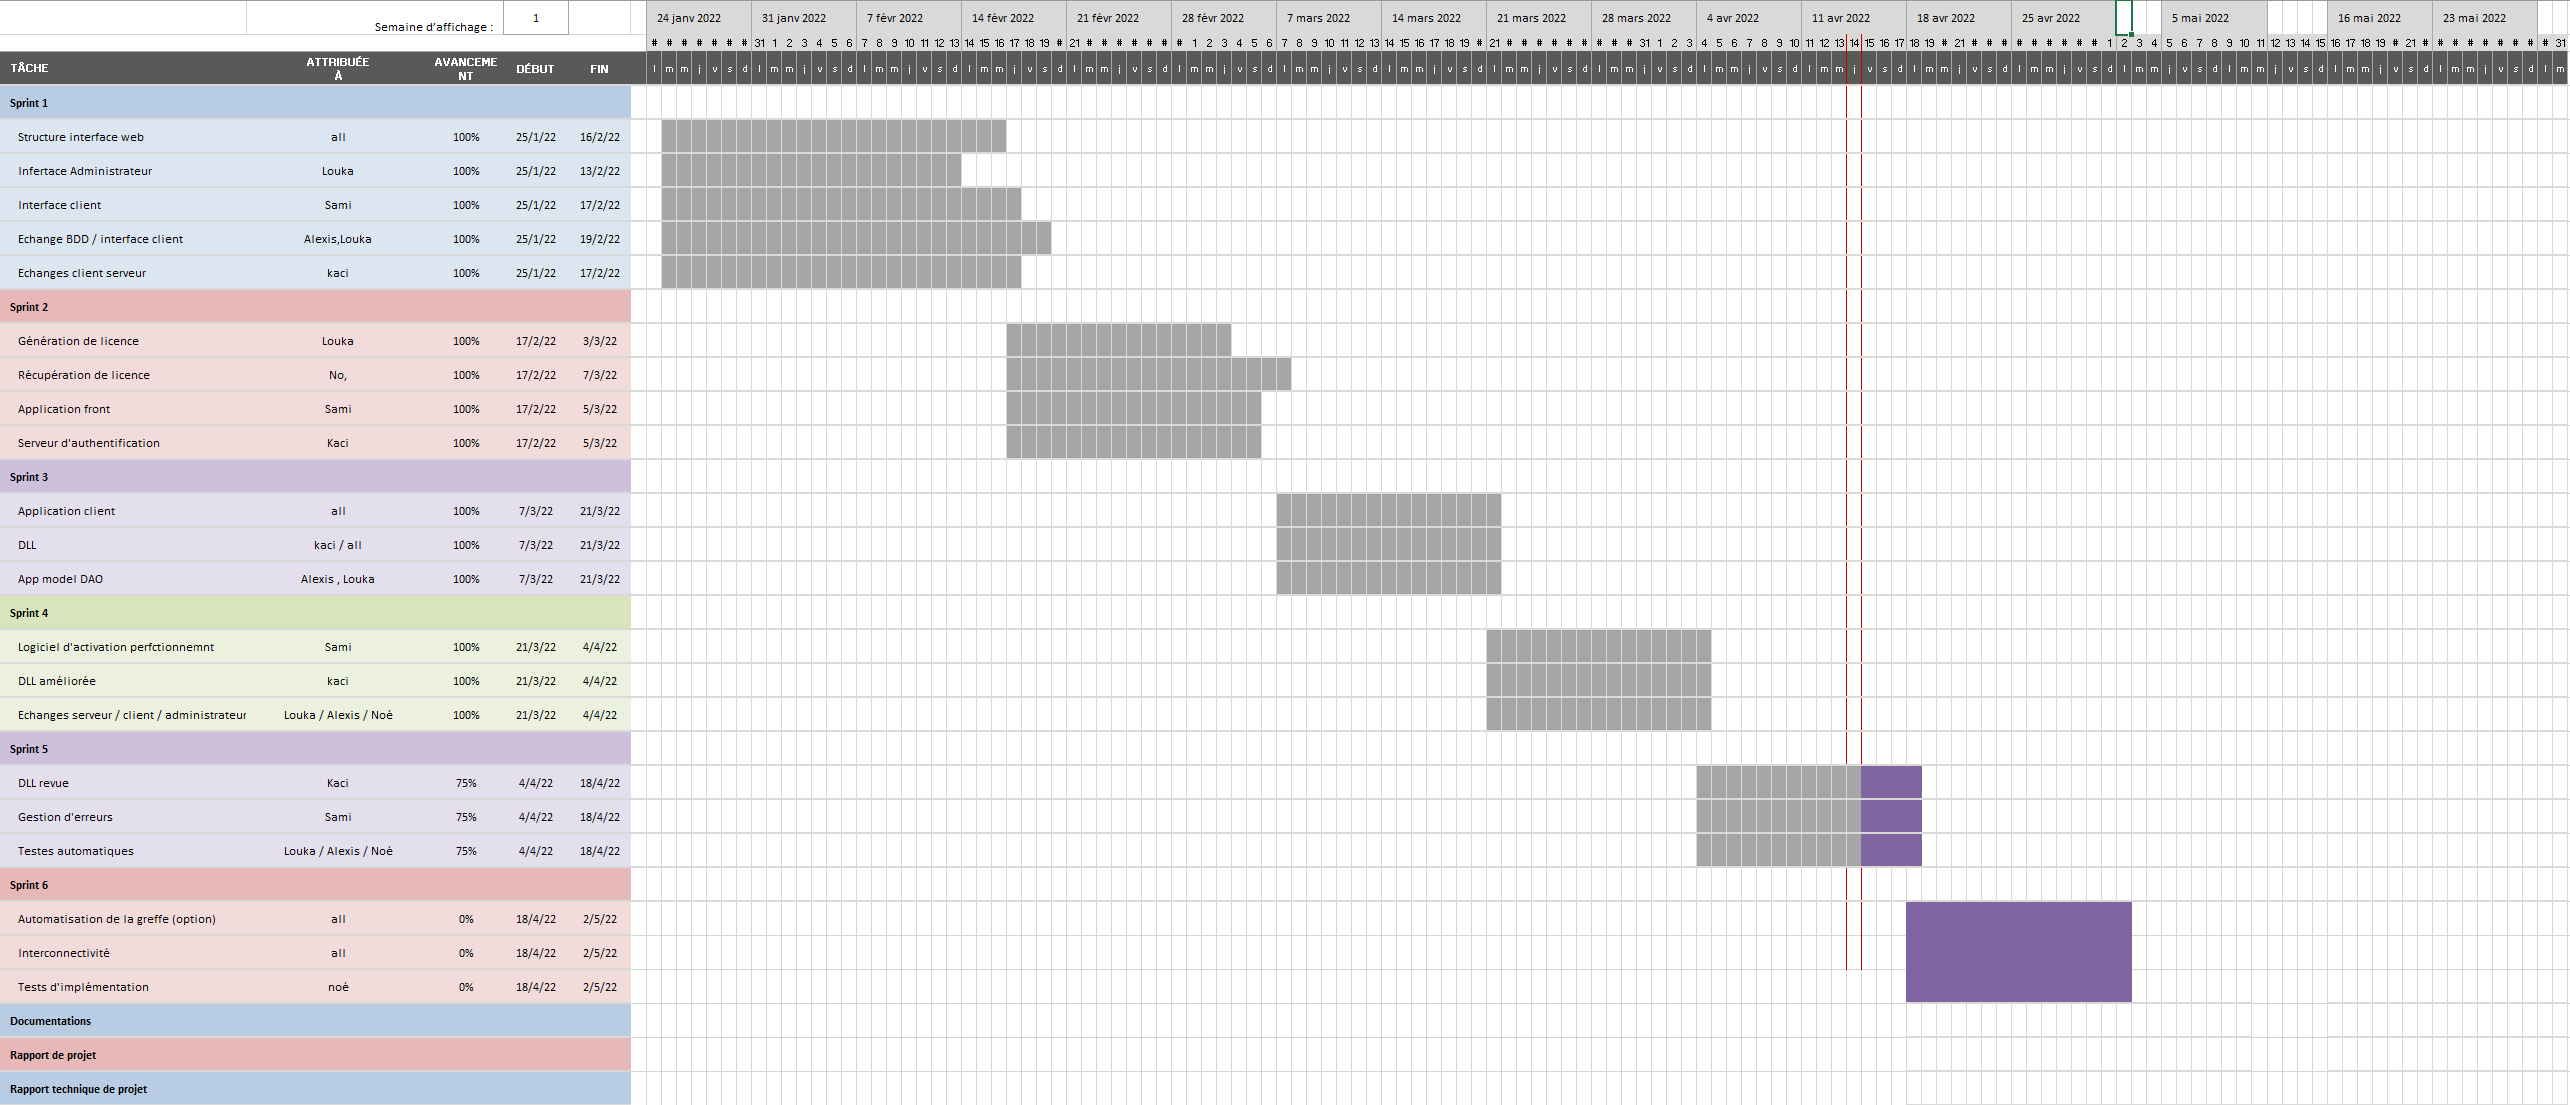
\includegraphics[width=15cm]{Gantt.png}
\end{figure}

La phase de développement du projet a donc, si nous nous referons aux anciennes estimations, suivis son cours.\newline

Celle-ci s'est donc découpé en phase de sprint de 2 semaines chacune. Chaque sprint se décomposé de la manière suivante :\newline  

\begin{itemize}
	\item 1 - Réunion de debut de sprint avec l'équipe pour faire une estimation de temps de taches définies ainsi que pour les attribuer.\newline
	\item 2 - Réunions journalière pour faire le point sur les avancés et les blocages de la veille.\newline
	\item 3 - Réalisation des taches définies.(Développement)\newline
	\item 4 - Réunion de fin de sprint (Sprint Review) avec le client pour nous donner son retour sur l'itération précédente, et démonstration faites au cours de la réunion.\newline
	\item 5 - Fin de réunion pour confirmer les prochains livrables et les dates.\newline
	\item 6 - Livraison du livrable au client.\newline
	\item 7 - Retrospective du sprint sur RetroMetro (outil de retrospective). Cette phase permet de mettre en lumière les éléments/actions positives qui font avancer le projet ou à l'inverse ceux qui l'entrave. 
\end{itemize}

Pour avancer rapidement et efficacement, nous avons
continué d’utiliser diverses plateformes en en avons ajouté de nouvelles:\newline

\begin{itemize}
	\item Discord :\\
	Cet outil nous permet de communiquer rapidement entre nous et
    de faire des audios / visioconférences pour nos réunions. Il est aussi très utile
    pour communiquer rapidement et faire des annonces importantes (réunions,
    vérification d’un mail avant son envoi, etc.) et pour partager / archiver les
    comptes rendus de toutes les réunions.\\
	
    \item Trello :\\
	Cet outil nous permet de répartir et de savoir sur quelle tâche
    travaillent les membres de l’équipe et de connaître leur avancement.\\
    
    \item RetroMetro :\\
    Est un tableau blanc en ligne favorisant l’expression et le travail entre membres d’une même équipe 
    à distance ou même sur une même machine.Cet outil un excellent moyen de susciter toute l'équipe pour
    que tous puisse relever les bons comme les mauvais points du sprint au moment du sprint retrospective\\

    \item GitHub :\\
	L’université nous a fourni cet outil qui est très pratique pour stocker
    les documentations produites et le code source de l’application que nous
    aurons à faire lors de la phase de développement.Cette outil a aussi été utilisé pour son outil de visualisation des taches effectuées
		ce qui nous permis de créer des BurnDown Chart afin de relever les erreurs de planning ou de répartition de taches\\
	
    \item Google docs / GitHub :\\
	Ces outils nous permettent de réaliser les documents demandés
    pour la matière Gestion de Projet. Google Docs nous permet de travailler à
    plusieurs sur un même document. Les modifications apparaissent en temps
    réel et sont sauvegardées sur une période de trente jours. Il est donc possible
    de consulter des versions antérieures de nos documents en quelques clics.\\

		\item BigBlueButton :\\
		Outils de télécommunication préféré par le client pour effectuer les sprint review lors de ses déplacement.	


\end{itemize}

\chapter{Implémentation}

\section{Licence}

L'un des éléments les plus important du projet sont les fichiers de licence.
\newline
Ils doivent pouvoir contenir toutes les informations concernant les droits d'un
utilisateur sur un logiciel, tout en garantissant qu'il ne pourra pas être 
modifié par l'utilisateur après avoir été distribué par le fournisseur.
\newline

Le fichier de licence étant utilisé par de nombreux acteurs dans le projet, 
nous avons décidé d'utiliser le format JSON afin qu'il puisse ête lu peu importe
la plateforme. JSON étant conçu dans ce but.
Ainsi le contenu de la licence est formatée sous forme d'un JSON. Nous reviendront
sur les différentes clés du json par la suite.
\newline

Ce json est ensuite encodé en base64 afin de pouvoir être signé sans soucis 
d'interprétation vis à vis des espaces et retours à la ligne dans le cas où nous 
aurions signé le json directement.
\newline

Le base64 va donc être signé en utilisant l'algorithme bcrypt avec la clé privée 
du fournisseur. Le résultat étant un binaire, il sera lui aussi encodé en base64 
afin d'être copié sans soucis sous format texte dans le fichier de licence. 
\newline

Puis ces deux éléments seront mis en forme entre des headers permettant de 
partager le fichier de licence en plusieurs partie. Si ce format n'est pas 
respecté la DLL ne pourra pas lire le fichier.
\newline

Ainsi au moment de la vérification, la DLL pourra récupérer le base64 du contenu 
de la licence et le base64 de la signature. Décoder la signature et la vérifier.
Si la signature est bonne, décoder le JSON et en exploiter le contenu.

\section{DLL}

La DLL est composée de 3 éléments principaux. LicenceChecker, Licence(Wrapper) 
et MachineHardware.\newline

MachineHardware contient les fonctions de génération d'identifiants machine 
uniques. Ces derniers sont générés à partir des composants materiels de la 
machine et il est possible de ne sélectionner que certains composants et pas 
d'autres. La liste des composants pris en charge sont : Le processeur, 
la carte mère, le bios, le disque dur et les cartes réseaux. Ce sont les numéros
de série et adresses mac qui sont pris en compte.\\ 
Cet identifiant sera par la suite ajouté au fichier de licence permettant de 
cibler une machine précise et de faire en sorte que la licence ne puisse pas 
être utilisé autre part.\\
De plus, le module prend en compte une clé anti fraude qui est générée 
aléatoirement et qui est stockée dans la base de registre. Dans le cas où cette 
clé existe, le module l'utilisera afin de l'intégrer dans les identifiants 
Machine. Si elle n'existe pas, le module la génère la stock et l'utilise. Cela 
donnera ainsi un identifiant machine différent et invalidera les fichiers de 
licences précédemment générés.
\newline

Licence dans les fichiers sources ou LicenceWrapper est une classe permettant 
d'englober au niveau objet un fichier de licence. Celui ci se charge de lire le 
fichier et d'en extraire le contenu tout en y vérifiant le formatage. 
Un formatage particulier est attendu. Ensuite l'objet de classe Licence est mis
à disposition dans LicenceChecker afin d'être utilisé. Les attributs disponibles
sont par exemple la date de validité, l'identifiant de la machine ciblée, le nom
du logiciel protégé etc, ces clés sont bien sûr modulables et peuvent évoluer au 
fil du temps afin d'ajouter de nouvelles conditions.
\newline

Une fois le fichier de licence parsé, nous pouvons verifier si toutes les 
conditions sont réunies afin de pouvoir lancer le logiciel. Cela est donc fait 
dans LicenceChecker qui va se charger d'effectuer tous ces tests et de fournir 
une api au développeur afin qu'il puisse facilement verifier les différents 
aspects de la licence.
\newline

Nous pouvons vérifier l'intégrité de la licence en vérifiant la signature, 
permettant de détecter si le contenu de la licence a été modifiée. Il est 
possible d'accéder aux différents attributs de la licence, et de vérifier 
point par point au bon vouloir du développeur la validité de la licence.\\
Ce module inclut aussi les fonctions de détection de fraude. En effet ce 
dernier enregistre la date de dernier lancement du logiciel, afin de pouvoir 
tester au prochain lancement que la date et l'heure de la machine n'ai pas été
modifiée. Si c'est le cas, le module se chargera de supprimer la clé de registre
servant à générer l'identifiant machine, faisant que la licence devient 
à présent inutilisable.

\chapter{Système}

Nous avons choisi en accord avec monsieur Macadré de créer 2 machines virtuelle qui héberge donc nos serveur. L'une est utilisée en tant que machine de gestion de licence 
et l'autre en tant que serveur de web qui gère toute cette partie afin d'acheter ces même licences par exemple.\newline

Les machines virtuelles d'authentification et de web se composent donc de quelques éléments :\newline

\begin{itemize}
	\item Un serveur Tomcat pour héberger notre site
	\item Une architecture au format MVC soutenue par le model DAO (vu au premier semestre)
	\item Une connexion en ssh pour pouvoir gérer ce périphérique
	\item Un nom de domaine valide. (Pour être disponible en accès à l'université ou depuis un poste extérieur grâce au VPN)\newline
\end{itemize}

Étant en M1 sécurité des systèmes d'information il était de notre devoir d'administrer ces machines de manière sécurisée.
C'est pourquoi nous avons donc défini des comptes ayant des droits restreint pour limiter les accès en contenant les développer au strict nécessaire.
De plus au moment de la création des comptes les normes données par l'ANSI ont été respectées.

\section{Machine virtuelle d'authentification}

\section{Machine virtuelle web}

\chapter{Problèmes rencontrés}

\section{Gestion de projet}

Durant ce projet nous avons rencontrés plusieurs problèmes en termes de gestion de projet comme évoqué précédemment.
Nos points de progression, ou les choses à faire autrement si l'on devait refaire le projet sont les suivants :
\begin{description}
    \item[Amélioration de la communication]
        Aussi bien entre nous, qu'avec le client, nous avons eu des soucis de communication et par conséquent cela
        a créer des incompréhensions sur la répartition des tâches, les priorités du client ou encore la compréhension
        du projet par chacun. Des réunions plus régulières (style daily-meeting) nous auraient permis de nous assurer
        que chacun possède une tâche, comprends ce qu'il doit faire etc...
    \item[Modification des priorités]
        Une meilleur communication nous aurez permis de mieux cerner les besoins du client et ainsi de pouvoir ordonner
        les tâches autrement. Notamment, le développement de la plateforme Web nous a pris beaucoup de temps (pour qu'elle
        soit fonctionnel, ergonomique et sécurisé) et donc forcément, nous avons eu moins de temps pour la partie vérification
        de la licence : la bibliothèque et l'injection de code, alors que c'était ce que le client souhaitait en priorité.
    \item[Revoir l'estimation]
        Nous avons été très optimiste quant à l'estimation du temps nécessaire à la réalisation du projet. Si nous devions
        revoir l'estimation, il faudrait prévoir plus de temps pour chaque tâche et en particulier pour les parties qui 
        nous étaient inconnues. Par exemple pour l'injection de code et l'obfuscation nous aurions dû prévoir du temps
        pour comprendre le mécanisme avant d'essayer de le faire.
\end{description}

\section{Partie technique}

\begin{description}
    \item[Utilisation de framework]
        Étant donné que la partie développement n'était pas censé être au centre du projet si nous avions utilisé un/des
        framework(s) pour cela, nous aurions pu faire ça plus rapidement et passer aux tâches suivantes.
    \item[Poursuivre la greffe de code]
        Si l'on avait fait tous les améliorations précédentes nous aurions donc pu au final passer plus de temps sur 
        l'injection de la vérification de licence dans les exécutables des logiciels du client. Cela nous aurait aussi
        permis d'essayer quelques techniques d'obfuscation, afin d'apporter plus de sécurité à notre solution.
    \item[Améliorer le système de détection de fraude]
        Le système de détection de fraude concernant la validité de la licence est fonctionnel et permet de corriger
        potentiels failles qu'un utilisateur lambda pourrait utiliser pour outre-passer la vérification de la licence
        (par exemple modifier le fichier de licence ou l'heure). Cependant le système n'est pas assez robuste pour
        empêcher un utilisateur expérimenté et motivé d'obtenir une licence pour un temps plus long que celui défini
        dans la licence. Cette détection pourrait être améliorer (voir POC sur la détection de fraude avec la date).
\end{description}

\chapter{Retour d'expérience}

\section{Partie technique}
    Programmation :\\
    \newline
    En effet au cours de ce projet nous avons appris à coder en C\#, partant de zéro pour la plupart des membres du groupe, 
    cela a été une expérience de plus à ajouter à nos compétences acquises. Nous avons par ailleurs confirmer des sujets abordés 
    au premier semestre, tel que le développement sous le modèle DAO.
    \newline

     Connaissances sur les techniques d'injection de code :\\
    \newline
    Malgré le fait que nous n'avons pas réussi à implémenter l'injection de code définie dans la phase de préparation, 
    néanmoins nous avons passé un temps non négligeable sur ce sujet. Tout le système de recherche et toutes les tentatives pour 
    tenter de le faire fonctionner nous aurons tout de même servis à en apprendre plus sur l'injection de code et ce qui l'entoure.
    \newline

     Mise en place d'un système composé de plusieurs éléments :\\
     \newline
     Le coeur du projet étant de réaliser un gestionnaire de licence il a donc été nécessaire de diviser les parties. 
     Cette division a donné lieu à des connexions afin d'échanger des informations et des données entre ces parties. 
     Nous en avons appris beaucoup sur la connectivité et les échanges de données, c'est pourquoi nous plaçons cette partie en tant  qu'expérience.
     \new line
    
     Mise en pratique d'outils cryptographiques :\\
     \newline
     Au cours du premier semestre nous avons suivi les enseignements de cryptographie, ces enseignements ont été mis en pratique ce semestre avec le système de signature de la licence ou celui de 
     El Gamal que nous avons voulu implémenter nous-mêmes sans réaliser l'ampleur de la tâche et ses difficultés.
     \newline
     \newpage
\section{Partie Gestion de projet}
    Compétences en gestion de projets : \\
    \newline
    Pour certain d'entre nous le parti gestion de projets n'était pas essentiel pour mener à bien notre projet. Réaliser le projet en 
    mettant en place des outils de gestion tel que Trello / Git / RetroMetro nous aura été d'une utilité inespérée. 
    À la fin de ce projet nous ressortirons donc avec des compétences quant à l'utilisation de ces outils et leurs compréhensions.
    \newline

    Communication \& Organisation : \\
    \newline
    L'audit et la partie sprint rétrospective nous ont permis de réaliser certains problèmes et d'y trouver des solutions. Le fait de communiquer 
    n'était pas acquis pour certain, c'est pourquoi grâce aux méthodes de gestion et aux outils disponible, nous avons permis à tous de communiquer 
    ce qui est l'atout principal de l'organisation et du bon déroulement du projet.
    \newline

    Gestion d'un client :\\
    \newline
    Avoir un client à des points négatifs et positifs. Le retour d'expérience sur le fait d'avoir un client est complexe mais nécessaire. En effet nous avons appris au fur et 
    à mesure, à comprendre et anticiper les demandes et les attentes de notre client. Quant à la partie gestion nous avons mis en place des systèmes de compte rendu de réunion et de rapport post-réunions pour indiquer au client les sujets abordés lors 
    de la prochaine réunion. De plus cela nous aura appris à réaliser un projet sous contrainte constante contrairement à l'université.

\chapter{Conclusion}

    Pour conclure ce rapport, ce projet aura été bénéfique sur plusieurs plans.
    Techniquement nous avons tous évolué, comme dit précédemment, nous avons 
    abordé des points que nous n'avions jamais eu l'occasion d'aborder.\\

    Professionnellement, cette expérience nous a rapproché du monde du travail 
    et de ses contraintes. Notamment dans le fait de prévoir un planning et de 
    s'y tenir, mais aussi de gérer des effectifs humains.\\
    
    Au niveau de la réussite du projet, lors de notre dernière entrevue avec le 
    client, nous avons pu obtenir la confirmation de sa satisfaction. Le projet
    à l'heure actuel est fonctionnel et pourrait être utilisé tel quel. Bien sûr,
    ce dernier contient toujours des failles et il en contiendra sûrement 
    toujours étant donné la complexité de la tache et de toutes les manières 
    possibles de contourner ce genre de système, néanmoins nous sommes sûr que 
    les sécurités mises en place seront suffisantes compte tenu du niveau 
    informatique des utilisateurs des logiciels du client.\\

    Nous espérons que ce projet pourra être repris par un potentiel futur groupe 
    d'étudiant afin d'être complété, amélioré et maintenu.\\

    Nous tenons à remercier l'ensemble de l'équipe pédagogique pour tous ces 
    enseignements.

    \label{chapter:bilan}

